\documentclass[conference]{IEEEtran}
\IEEEoverridecommandlockouts
\usepackage{cite}
\usepackage{amsmath,amssymb}
\usepackage{graphicx}
\usepackage{textcomp}
\usepackage{xcolor}
\usepackage{booktabs}
\usepackage{url}
\usepackage{tikz}
\usetikzlibrary{positioning,arrows.meta,fit,backgrounds}
\def\BibTeX{{\rm B\kern-.05em{\sc i\kern-.025em b}\kern-.08em T\kern-.1667em\lower.7ex\hbox{E}\kern-.125emX}}

% --- house colours, muted for print ---
\definecolor{ink}{HTML}{04201D}
\definecolor{teal}{HTML}{00776A}
\definecolor{soft}{HTML}{00A693}
\definecolor{rule}{HTML}{C9D8D5}

\begin{document}

\title{Suvana: An Integrated Platform for Two-Way\\
Deaf--Hearing Communication in Sri Lankan Sign Language}

\author{
\IEEEauthorblockN{R.M.LK.~Chamara}
\IEEEauthorblockA{\textit{Dept. of Software Engineering}\\
\textit{SLIIT}\\
Malabe, Sri Lanka\\
it22076816@my.sliit.lk}
\and
\IEEEauthorblockN{G.W.L.~Malkith}
\IEEEauthorblockA{\textit{Dept. of Software Engineering}\\
\textit{SLIIT}\\
Malabe, Sri Lanka\\
it22630834@my.sliit.lk}
\and
\IEEEauthorblockN{T.P.K.~Gimhan}
\IEEEauthorblockA{\textit{Dept. of Software Engineering}\\
\textit{SLIIT}\\
Malabe, Sri Lanka\\
it22266996@my.sliit.lk}
\and
\IEEEauthorblockN{R.A.K.N.~Ranathunga}
\IEEEauthorblockA{\textit{Dept. of Software Engineering}\\
\textit{SLIIT}\\
Malabe, Sri Lanka\\
it22552860@my.sliit.lk}
\and
\IEEEauthorblockN{Hansi De Silva}
\IEEEauthorblockA{\textit{Dept. of Software Engineering}\\
\textit{SLIIT}\\
Malabe, Sri Lanka}
\and
\IEEEauthorblockN{Ishara Weerathunga}
\IEEEauthorblockA{\textit{Dept. of Software Engineering}\\
\textit{SLIIT}\\
Malabe, Sri Lanka}
}

\maketitle

\begin{abstract}
Sri Lankan Sign Language (SSL) is documented as under-served: interpreter
provision is limited, no fully standardised national variety exists, and
sign-language technology overwhelmingly targets American Sign Language. We
present \emph{Suvana}, a platform that brings four SSL components under one
deployment: isolated sign recognition with Sinhala speech output, Sinhala
speech to a signing avatar, on-device ambient-sound alerting, and an
in-browser practice tutor for hearing learners. Our contribution is twofold.
First, we describe an integration topology that lets four independently
developed research prototypes --- three web applications, one mobile
application and two Python services --- be served as a single product without
merging their codebases, including a documented exception for the component
whose transport cannot be proxied. Second, we report a calibrated
Dynamic Time Warping (DTW) grader for the practice module and give measured
evidence that open-set identification on the same distance metric would be
unsafe: the closest pair of \emph{distinct} SSL signs in our reference library
sits $0.135$ apart in normalised hand-size units, while two correct renditions
of the \emph{same} sign sit a median $0.458$ apart. We therefore grade a
specified sign rather than classify an unknown one. We report the practice
module's discrimination as ROC~AUC~$0.744$ against a $65.4\%$ majority-class
baseline, and state explicitly which of our targets remain unmeasured. We
also report the recognition module's accuracy under the signer-dependent
protocol it was trained with, and decline to interpret it as generalisation
performance. All four authors are hearing; no Deaf signer has yet validated
any component, and we set out what that means for the claims we make.
\end{abstract}

\begin{IEEEkeywords}
Sri Lankan Sign Language, low-resource sign languages, dynamic time warping,
sign language tutoring, accessibility, system integration
\end{IEEEkeywords}

% =========================================================================
\section{Introduction}

Udugama \emph{et al.}~\cite{udugama2024sign}, surveying deaf and
hard-of-hearing provision across all nine provinces of Sri Lanka, report that
the country ``lacks a fully developed common sign language,'' that interpreter
shortages are severe, and that deaf Sri Lankans remain ``marginalized,
under-supported.'' A recent review of a decade of SSL technology
work~\cite{ahinsa2025comprehensive} identifies persistent obstacles of the
same shape: small datasets, regional sign variation, absent linguistic
standards, and a lack of expressive synthesis. The two published SSL
recognition systems we could locate~\cite{thennakon2025realtime,
herath2022approach} both address recognition alone.

We do not claim to remove a communication barrier. Desai
\emph{et al.}~\cite{desai2024systemic}, in a Deaf-led review of 101 sign
language AI papers, name exactly that framing as the field's most common
bias, and we take the point. What we claim is narrower and technical: that
four separately built SSL prototypes can be operated as one product, and that
one of them --- a practice tutor --- can be calibrated against measured data
and characterised honestly.

\textbf{Contributions.}
\begin{enumerate}
\item An integration topology (Sec.~\ref{sec:arch}) under which four
prototypes with incompatible stacks share one origin, one visual identity and
one account, without codebase merging, and with the one transport-level
exception documented rather than hidden.
\item A DTW-based grader for SSL practice whose distance-to-score map is
\emph{fitted} to measured data rather than assumed, and whose feature
weighting was chosen against, not with, the metric that a classification
objective would have maximised (Sec.~\ref{sec:learn}).
\item Measured evidence that the same distance metric cannot safely support
open-set identification, which motivates grading a specified sign instead of
recognising an unknown one (Sec.~\ref{sec:eval-learn}).
\item A staged evaluation statement that separates what is measured from what
is instrumented but not yet measured, and a positionality statement
(Sec.~\ref{sec:limits}) covering the absence of Deaf involvement.
\end{enumerate}

% =========================================================================
\section{Related Work}

\subsection{Sign language recognition for low-resource languages}
Landmark-based pipelines --- pose estimation followed by a sequence model ---
now dominate isolated recognition for languages without large corpora.
Alyami \emph{et al.}~\cite{alyami2024isolated} extract MediaPipe hand and face
keypoints for Arabic SL and compare LSTM, temporal convolution and
transformer heads; De Coster \emph{et al.}~\cite{decoster2023towards} show
that keypoint normalisation and missing-keypoint imputation materially improve
transfer for Flemish SL, and that keypoint models generalise across signers
better than image models. Shahgir \emph{et al.}~\cite{shahgir2024connecting}
report the same framing for Bangla SL, where a word-level dataset of 611
videos over 40 words was, at the time, the first of its kind. The SSL work we
found~\cite{thennakon2025realtime, herath2022approach} follows the same
landmark-plus-LSTM pattern.

\subsection{Evaluation protocol}
\label{sec:rw-protocol}
The benchmark literature is unambiguous that signers must be disjoint across
splits. AUTSL~\cite{sincan2020autsl} was built so that ``the signers in the
test set do not appear in the training set,'' and reports, on identical data
and models, $95.95\%$ under a random split against $62.02\%$ under the
user-independent benchmark. MS-ASL~\cite{vaezijoze2019msasl} is designed for
the same reason. Alyami \emph{et al.}~\cite{alyami2024isolated} report
$99.74\%$ signer-dependent against $68.2\%$ signer-independent on KArSL-100.
FluentSigners-50~\cite{mukushev2022fluentsigners} publishes three splits and
urges reporting on the signer-independent one. Akdag and
Baykan~\cite{akdag2024enhancing} report three protocols side by side, and
Podder \emph{et al.}~\cite{podder2023signer} demonstrate that leave-one-signer-out
cross-validation is viable with as few as four signers. Pal \emph{et
al.}~\cite{pal2023importance} argue the general principle that controlling
for overlap is required for a realistic estimate. Separately,
WLASL~\cite{li2020word} shows top-1 accuracy falling from $65.89\%$ at 100
glosses to $32.48\%$ at 2000, which bounds what is plausible at any given
vocabulary size. Section~\ref{sec:eval-recognise} states where our own
recognition result sits against this literature.

\subsection{Deaf participation}
Bragg \emph{et al.}~\cite{bragg2019sign} open their interdisciplinary
workshop report with the call to ``involve Deaf team members throughout,'' and
state that ``an all-hearing team lacks the lived experience of Deafness.''
Desai \emph{et al.}~\cite{desai2024systemic} find the field ``dominated by
hearing non-signing researchers'' and warn that claimed Deaf collaboration has
itself become tokenising. De Meulder~\cite{demeulder2021good} argues the
ideologies behind these technologies need interrogation; De Meulder \emph{et
al.}~\cite{demeulder2024lessons} distinguish co-creation from ``participation
as consultation,'' where deaf users are positioned as testers of pre-built
systems. Bragg \emph{et al.}~\cite{bragg2021fate} set out dataset ethics,
including community claims to ownership of sign language data. The WFD and
WASLI~\cite{wfdwasli2018avatars} caution against signing avatars as a
replacement for human signers, permitting narrow use only for pre-recorded
static content and only where deaf people have advised on the signed
sentences. Yin \emph{et al.}~\cite{yin2021including} argue for treating signed
languages as full natural languages rather than gesture-to-word maps, and
Angelini \emph{et al.}~\cite{angelini2025speculating} report what deaf
participants themselves ask of technology. We return to all of this in
Sec.~\ref{sec:limits}.

% =========================================================================
\section{System Architecture}
\label{sec:arch}

Suvana is a monorepo of four applications and three supporting services
(Fig.~\ref{fig:arch}). The four were built independently, in different
stacks, before integration: a static shell, a React single-page application,
a Next.js full-stack application, a React Native mobile application, and two
Python services. The integration constraint was therefore to present one
product without rewriting any of them.

\begin{figure}[t]
\centering
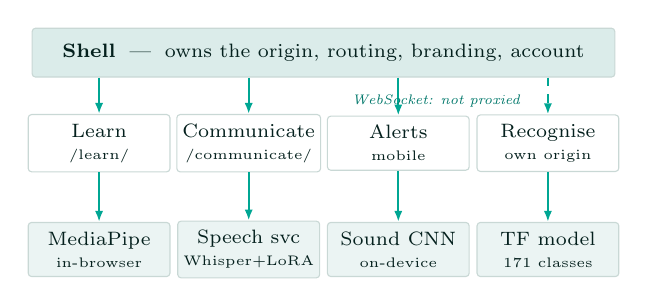
\begin{tikzpicture}[
  font=\scriptsize,
  box/.style={draw=rule, fill=white, rounded corners=1.2pt, minimum height=6.2mm,
              align=center, inner xsep=2pt, text=ink},
  mod/.style={box, minimum width=18mm},
  svc/.style={box, minimum width=18mm, fill=teal!8},
  lbl/.style={font=\tiny\itshape, text=teal},
  ar/.style={-{Latex[length=1.4mm]}, draw=soft, thick}
]
\node[box, minimum width=74mm, fill=teal!14] (shell) at (0,0)
  {\textbf{Shell} \;---\; owns the origin, routing, branding, account};

\node[mod] (learn)  at (-2.85,-1.15) {Learn\\\tiny{/learn/}};
\node[mod] (comm)   at (-0.95,-1.15) {Communicate\\\tiny{/communicate/}};
\node[mod] (alerts) at ( 0.95,-1.15) {Alerts\\\tiny{mobile}};
\node[mod] (recog)  at ( 2.85,-1.15) {Recognise\\\tiny{own origin}};

\draw[ar] (shell.south -| learn.north)  -- (learn.north);
\draw[ar] (shell.south -| comm.north)   -- (comm.north);
\draw[ar] (shell.south -| alerts.north) -- (alerts.north);
\draw[ar, dashed] (shell.south -| recog.north) -- (recog.north);

\node[svc] (mp)   at (-2.85,-2.5) {MediaPipe\\\tiny{in-browser}};
\node[svc] (sp)   at (-0.95,-2.5) {Speech svc\\\tiny{Whisper+LoRA}};
\node[svc] (snd)  at ( 0.95,-2.5) {Sound CNN\\\tiny{on-device}};
\node[svc] (tf)   at ( 2.85,-2.5) {TF model\\\tiny{171 classes}};

\draw[ar] (learn)  -- (mp);
\draw[ar] (comm)   -- (sp);
\draw[ar] (alerts) -- (snd);
\draw[ar] (recog)  -- (tf);

\node[lbl, anchor=east] at (2.62,-0.62) {WebSocket: not proxied};
\end{tikzpicture}
\caption{Suvana's topology. The shell owns the domain root and proxies three
modules by path prefix. Recognise (dashed) runs on its own origin because
WebSocket upgrades cannot pass through the platform's path rewrites.}
\label{fig:arch}
\end{figure}

\textbf{One origin, four prefixes.} The shell owns the domain root. Learn
builds with a Vite \texttt{base} of \texttt{/learn/}; Communicate runs with a
Next.js \texttt{basePath} of \texttt{/communicate}, which namespaces its
pages, assets and API routes together. Platform-level rewrites forward each
prefix to its own deployment. Unsetting the base path variable collapses
Communicate to standalone behaviour, so integration is reversible.

\textbf{The exception, stated.} Recognise streams camera frames over a
WebSocket. Path rewrites on our deployment platform do not proxy WebSocket
upgrades, so Recognise runs on its own origin and serves its own frontend. We
report this rather than describing a uniformity the system does not have; it
is the kind of detail that determines whether an integration claim is
reproducible.

\textbf{Client-side asset paths.} Under a base path, a bare absolute fetch
bypasses the prefix. Learn resolves runtime asset paths through the build
tool's injected base URL, and Communicate routes API calls through a helper
rather than string literals. Both are integration couplings that a naive
re-sync from an upstream standalone repository silently removes; we maintain
them as an explicit list.

% =========================================================================
\section{Components}

\subsection{Recognise --- signing to Sinhala speech}
\label{sec:recognise}
Camera frames are captured in the browser and streamed to a FastAPI service.
Per frame, MediaPipe yields a 1629-dimensional landmark vector; sequences of
30 frames are classified over 171 SSL gloss classes. The deployed classifier
is a stacked LSTM (256/128/64 units, followed by dense layers of 256 and 128
and a softmax), trained for 50 epochs with a batch size of 32 and a learning
rate of $10^{-3}$. A confidence threshold of $0.7$ and a smoothing window of
5 frames gate the output, which is spoken in Sinhala.

We note for accuracy that although the project's working title refers to
transformer models, the deployed sign classifier is recurrent; the only
transformer in the platform is the Whisper encoder-decoder in
Sec.~\ref{sec:communicate}. A transformer variant is scaffolded but untrained,
and we make no claim for it.

\subsection{Communicate --- Sinhala speech to a signing avatar}
\label{sec:communicate}
Audio is transcribed by \texttt{whisper-medium} with a Sinhala-fine-tuned LoRA
adapter, merged for inference and decoded greedily under a 96-token cap.
Transcripts are tokenised with a Sinhala tokeniser and mapped to SSL glosses
through a stored lexicon; a 3D avatar then renders the gloss sequence. A
prosody classifier is intended to condition delivery on speaker emotion.

Two statements of scope follow the WFD/WASLI
position~\cite{wfdwasli2018avatars}. First, the avatar's poses were authored
by hand by a hearing student and have not been reviewed by a Deaf signer; we
present the avatar as an illustration of the pipeline, not as validated SSL,
and we make no intelligibility claim. Second, at the time of writing the
trained prosody classifier artefact is not deployed, and the service falls
back to an off-the-shelf English model; we therefore report no emotion result
at all rather than one obtained from a language-mismatched model.

\subsection{Alerts --- ambient sound}
A convolutional classifier runs entirely on the handset over seven ambient
classes: car horn, crying baby, dog, wooden door knock, footsteps, glass
breaking and siren. The model ships in two forms, a 9.1\,MB ONNX graph and a
sharded browser-runtime model. Detection raises a visual and haptic alert
naming the sound; an escalation flow shares location. This component is a
mobile application rather than a web application because it requires
background notification, location and messaging capabilities.

\subsection{Learn --- practice with corrective feedback}
\label{sec:learn}
The learner selects a gloss, views a reference recorded by a fluent signer,
performs it to a webcam, and receives a score in $[0,100]$ with written
correction. All processing is in-browser; attempts are stored locally and no
video leaves the device.

\textbf{Features.} MediaPipe returns 21 landmarks per hand per frame. Each
frame is split into a \emph{handshape} block --- landmarks made wrist-relative
and divided by hand size --- and a \emph{trajectory} block, the wrist path,
centred and scaled, with aspect-ratio correction. Both are invariant to where
in frame the learner stands and how far from the camera.

\textbf{Alignment.} DTW aligns the attempt against the reference and returns a
mean per-frame distance $d$ in hand-size units. Time warping absorbs speed
differences, so a slow but correct rendition is not penalised for being slow;
pace is judged separately. Critically, DTW also returns an alignment path, so
a deviation is attributable to a specific joint at a specific moment --- which
is what makes ``your ring finger is over-extended'' expressible. A classifier
returns a label and a confidence, from which no such correction follows
without inventing it. Every attempt is additionally scored mirrored, and the
better result taken, so that a left-dominant learner performing a
right-handed reference is not penalised.

\textbf{Fitted score scale.} $d$ maps linearly to $[0,100]$ between anchors
$d_{100}=0.22$ and $d_{0}=0.77$. These are not chosen: they are the 10th and
90th percentiles of the measured distance between two correct renditions,
over 557 takes. The previous anchors were assumed values, and placed $d_0$
\emph{below} the median correct rendition, so that a genuinely correct attempt
scored zero. Calibrating against data is what exposed that.

\textbf{Weighting, chosen against the metric.} Handshape and trajectory are
combined at $0.8/0.2$. A grid search over 11 weightings on 24 signs peaks at
$78.6\%$ separation with all weight on handshape --- that is, with movement
discarded entirely. We ship $0.8$, at $74.2\%$. The search optimises ``is this
the same sign?'', a classification objective, whereas the scorer grades a sign
the learner was already asked for; movement is a phonological parameter of
SSL, and a scorer blind to it would award full marks to a learner with the
right handshape and the wrong movement. We took the measured gain to $0.8$
and stopped.

% =========================================================================
\section{Evaluation}

\subsection{Data}
The practice module's reference library holds 501 recordings over 490 distinct
glosses, drawn from two public corpora: 141 under CC0 and 360 under
CC BY-NC-SA 4.0. Landmark sequences are shipped; no corpus video is
redistributed, and a test fails if a reference lacks its licence record. All
calibration uses the CC BY-NC-SA corpus: 557 takes over 33 signs, of which 32
are usable, since one sign has a single take and cannot form a positive pair.
There is a single signer. The corpus labels itself --- two takes of one sign
are a correct rendition performed twice, and takes of different signs are a
wrong-sign attempt --- so no human annotation is involved and none is claimed.
This yields 524 positive and 992 negative pairs.

\subsection{Practice module: discrimination}
\label{sec:eval-learn}

\begin{figure}[t]
\centering
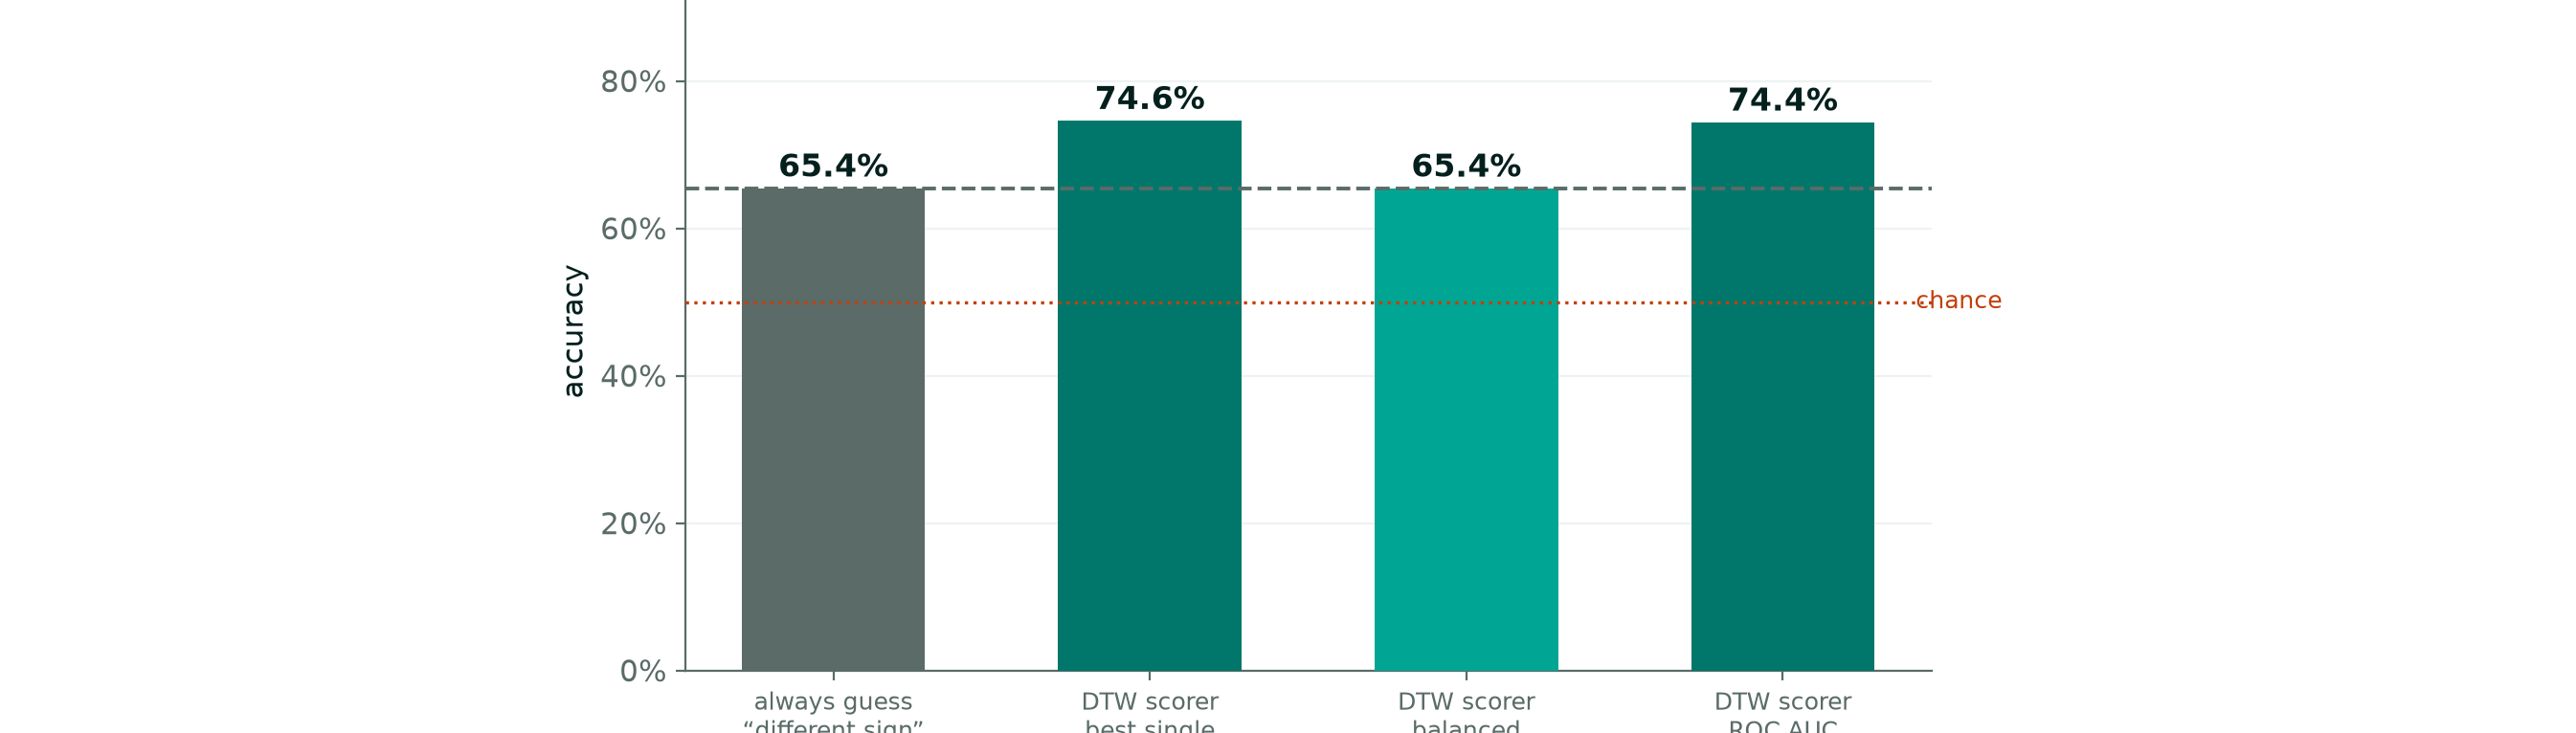
\includegraphics[width=\columnwidth]{figures/fig9-crop.png}
\caption{The distance metric's discrimination stated against its
majority-class baseline. Raw accuracy is reported only alongside the
baseline, because the pair set is imbalanced 524:992.}
\label{fig:baseline}
\end{figure}

Table~\ref{tab:learn} reports discrimination between a correct rendition and a
different sign. We lead with ROC AUC because it is threshold-free and
insensitive to the class imbalance; accuracy appears only beside its baseline
(Fig.~\ref{fig:baseline}). At the best single threshold the operating point is
$\mathrm{TPR}=0.357$, $\mathrm{FPR}=0.048$ --- the optimum buys accuracy by
rejecting, which is what an imbalanced set rewards, and one more reason the
product applies no threshold.

\begin{table}[t]
\caption{Practice module discrimination, 524 positive / 992 negative pairs}
\label{tab:learn}
\centering
\footnotesize
\begin{tabular}{lr}
\toprule
\textbf{Measure} & \textbf{Value}\\
\midrule
ROC AUC (threshold-free) & $0.744$\\
Majority-class baseline & $65.4\%$\\
Best single-threshold accuracy & $74.6\%$ at $d=0.370$\\
Gain over baseline & $+9.2$ points\\
Balanced accuracy at that threshold & $65.4\%$\\
Operational score gap (correct $-$ different) & $28.7$ points\\
Correct renditions scoring $\geq 50$ & $60.5\%$\\
Different signs scoring $\geq 50$ & $20.7\%$\\
\bottomrule
\end{tabular}
\end{table}

\textbf{Grading, not identifying.} Over 1766 distinct-sign pairs, the two
closest sit $0.135$ and $0.140$ apart, while the median distance between two
correct takes of the same sign is $0.458$. Some genuinely different signs are
therefore closer together than two correct renditions of one sign typically
are. A high score is not evidence that the right sign was made. This is a
property of the task, not a deficiency of the implementation, and it is why
the shipped system grades a sign the learner was asked for and never
identifies an unknown one. No threshold is applied anywhere in the deployed
system; the threshold in Table~\ref{tab:learn} is an evaluation device for
characterising the distance metric.

\textbf{What the learner sees.} On the shipped $[0,100]$ scale, correct
renditions average $56.7$ and different signs $28.0$, a gap of $28.7$ points.
This, not the AUC, is the quantity a user experiences.

\textbf{Cost.} The scoring stage --- DTW between a completed attempt and the
reference --- has a median cost of $1.8$\,ms and a 95th percentile of
$12.6$\,ms over $n=40$ references, against a $300$\,ms design budget. This
excludes landmark inference, framework commit and browser paint, and was
measured in Node rather than a participant's browser; it is not end-to-end
feedback latency, which is instrumented in the application but not yet
measured over enough real attempts to report.

\subsection{Recognition module: a protocol statement}
\label{sec:eval-recognise}
The recognition classifier records a test accuracy of $0.9878$ (loss $0.0532$)
over 171 classes. We report this as a \emph{signer-dependent} result obtained
under a random $0.2$ validation split, and we decline to present it as
generalisation performance.

Our reason is the literature summarised in Sec.~\ref{sec:rw-protocol}. On
identical data and models, AUTSL falls from $95.95\%$ to
$62.02\%$~\cite{sincan2020autsl} and KArSL-100 from $99.74\%$ to
$68.2\%$~\cite{alyami2024isolated} when signers are made disjoint. A figure in
the high nineties under a random split is what these systems report
immediately before that correction. WLASL~\cite{li2020word} independently
bounds what is plausible as vocabulary grows. We therefore treat a
signer-independent re-evaluation --- a fixed held-out signer set, or
leave-one-signer-out cross-validation following Podder \emph{et
al.}~\cite{podder2023signer} --- as required work before any generalisation
claim, and we report both figures side by side when it is done, as
in~\cite{akdag2024enhancing}.

\subsection{What is not measured}
Of four targets set for the practice module, one is measured. Feedback
latency is met at the scoring stage. Feedback agreement with expert judgment
is \emph{not} measured: the discrimination result above answers a different
question, and the target requires learner attempts graded by an SSL teacher,
which do not exist for SSL. Learning gain is instrumented --- every attempt
carries a session identifier --- but has zero participants. System usability
has neither participants nor a prepared instrument. The recognition,
communication and alerting components have no user-facing evaluation at all.

% =========================================================================
\section{Positionality and Limitations}
\label{sec:limits}

All four student authors are hearing, and none is a member of the Sri Lankan
Deaf community. We do not have the lived experience or the SSL fluency to
judge whether what this system produces or accepts is intelligible or
acceptable to Deaf signers. Bragg \emph{et al.}~\cite{bragg2019sign} state the
consequence directly: an all-hearing team ``lacks the lived experience of
Deafness, and is removed from the use cases and contexts within which sign
language software must function,'' and even hearing people with strong
community ties ``are not in a position to speak for Deaf needs.'' Mack
\emph{et al.}~\cite{mack2021what} find that $90.1\%$ of accessibility papers
with user studies included participants with disabilities; this work is in the
remaining minority.

We state the consequences without resolving them.

\emph{No Deaf validation.} No Deaf signer has reviewed any reference in the
library, any avatar pose, or any item of feedback text. Our reported numbers
measure agreement with corpus labels, not communicative adequacy.

\emph{Consultation is not co-design.} Our plan is to record references with a
teacher at a school for the Deaf. De Meulder \emph{et
al.}~\cite{demeulder2024lessons} name this tier accurately as participation as
consultation, with users positioned as testers of a pre-built system. We
describe it as that, and note that Desai \emph{et al.}~\cite{desai2024systemic}
warn that claimed Deaf collaboration has itself become tokenising.

\emph{Data provenance.} Both corpora are public and performed by real signers,
but neither was collected for this project and neither carries community
consent for this use. Bragg \emph{et al.}~\cite{bragg2021fate} record that
Deaf communities may claim ownership of sign language datasets. One corpus is
non-commercial by licence, which constrains what this project can become.

\emph{Which variety?} Sri Lanka lacks a fully standardised national
SSL~\cite{udugama2024sign}. A hearing team encoding one variety as canonical
is making a standardisation decision it has no standing to make. We invented
no vocabulary, gloss, handshape or sentence order at any point; every sign
comes from a published corpus.

\emph{Single signer.} All fitted constants derive from one fluent signer's
correct renditions. The measured spread is narrower than a learner's, so every
constant is optimistic. This locates the score scale; it does not substantiate
a grading-accuracy claim.

\emph{Non-manual markers.} The build tracks hands only, so facial expression,
head tilt and body movement are not captured. Their weight was reallocated
rather than scored as zero, and the deviation is disclosed in the application
itself. Treating signed languages as full natural
languages~\cite{yin2021including} requires these; we have not.

% =========================================================================
\section{Conclusion and Future Work}

We have described a platform that operates four SSL components as one product,
and a practice tutor whose scoring is calibrated against measured data rather
than assumed. The tutor's central design decision --- grading a specified sign
rather than identifying an unknown one --- is not a convenience but follows
from a measurement: distinct signs in our library can lie closer together than
two correct renditions of one sign.

The ordering of future work follows from what is unmeasured. First,
signer-independent re-evaluation of the recognition module. Second, a learner
study with expert grading, which is the only route to the agreement target and
would produce a corpus of SSL learner attempts, which does not currently
exist. Third, references recorded with, and validated by, Deaf signers ---
which bounds everything the scorer can do and is the precondition for treating
any output as authoritative. Fourth, restoring non-manual markers, which
requires face and pose tracking and a second calibration. Work with the Deaf
community should precede, not follow, further capability.

\section*{Acknowledgment}
The authors thank the School for the Deaf, Ratmalana. The reference corpora
are used under their respective licences; no corpus video is redistributed.

\bibliographystyle{IEEEtran}
\bibliography{references}

\end{document}
